\section{Project Pada Gitlab}

Pada bab sebelumnya kita telah mempraktekan pengoprasian apa saja yang dapat dilakukan pada github, seperti dengan membuat repository, membaca pull request, melakukan merge request dan sebagainya. Pada section kali ini kita kan mempelajari bagaimana pengoprasian pada gitlab. Pertama yang akan dijelaskan disini adalah bagaimana membuat project atau repository pada gitlab. 

Skenarionya sama dengan github dimana kita akan melakukan kontribusi terhadap sebuah project/repo \textit{Open Source} pada Gitlab. Pada dasarnya kita akan mempelajari bagaimana caranya untuk ikut berkontribusi kepada project \textit{Open Source} yang ada pada Gitlab. Untuk membantu para user yang baru memiliki akun gitlab, pertama-tama akan dijelaskan terlebih dahulu bagaimana melakukan setting konfigurasi key agar kita dapat mengakses semua project/repo dari profil kita. Berikut adalah langkah-langkah yang diperlukan untuk melakukan setting konfigurasi key :
\begin{enumerate}
\item Buat akun terlebih dahulu pada alamat \textbf{www.gitlab.com}
\item Install \textbf{Git Bash} dari alamat \textit{git-scm/downloads} pada komputer anda, kemudian buka aplikasi git bash setelah melakukan penginstallan.
\item Pastikan kita telah berada di \textit{home directory} dengan mengetikan perintah \textbf{cd} kemudian klik enter. Setelah itu untuk mengetahui posisi dimana direktori kita berada, ketikkan perintah \textbf{pwd} kemudian enter.
\item Lakukan proses generate key dengan perintah \textbf{ssh-keygen} seperti pada gambar \ref{fig:k1}
\subitem 
\begin{figure}[!htbp]
\centerline{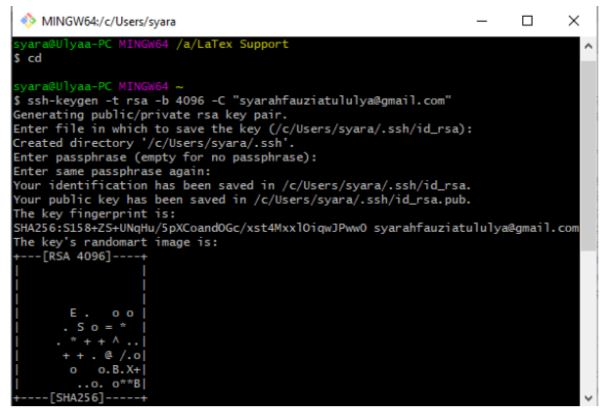
\includegraphics[width=.75\textwidth]{Figures/gitlab/SSH.JPG}}
\caption{Proses Generate Key Gitlab}
\label{fig:k1}
\end{figure}
\item Hasil outputnya seperti pada gambar \ref{fig:s1}
\subitem
\begin{figure}[!htbp]
\centerline{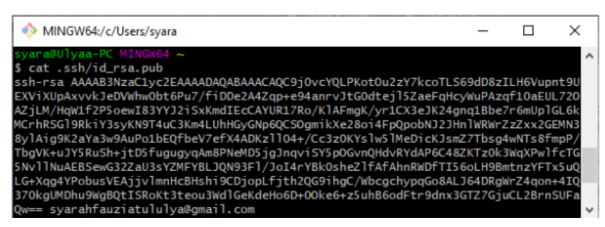
\includegraphics[width=.75\textwidth]{Figures/gitlab/SSH2.JPG}}
\caption{Hasil Output SSH Key Gitlab}
\label{fig:s1}
\end{figure}
\item Setelah melakukan proses tersebut, baca key yang sudah di generate dengan menggunakan perintah seperti pada gambar diatas 
\item Hasil output luaran yang sudah dibaca sebelumnya merupakan key yang kita miliki
\item Selanjutnya buka akun gitlab anda masing-masing masuk kebagian setting dan pilih menu \textbf{SSH KEY}
\item Terakhir copy-kan SSH Key pada gitbash yang sudah kita buat pada form seperti pada gambar \ref{fig:k2} lalu pilih button \textbf{Add key}
\subitem
\begin{figure}[!htbp]
\centerline{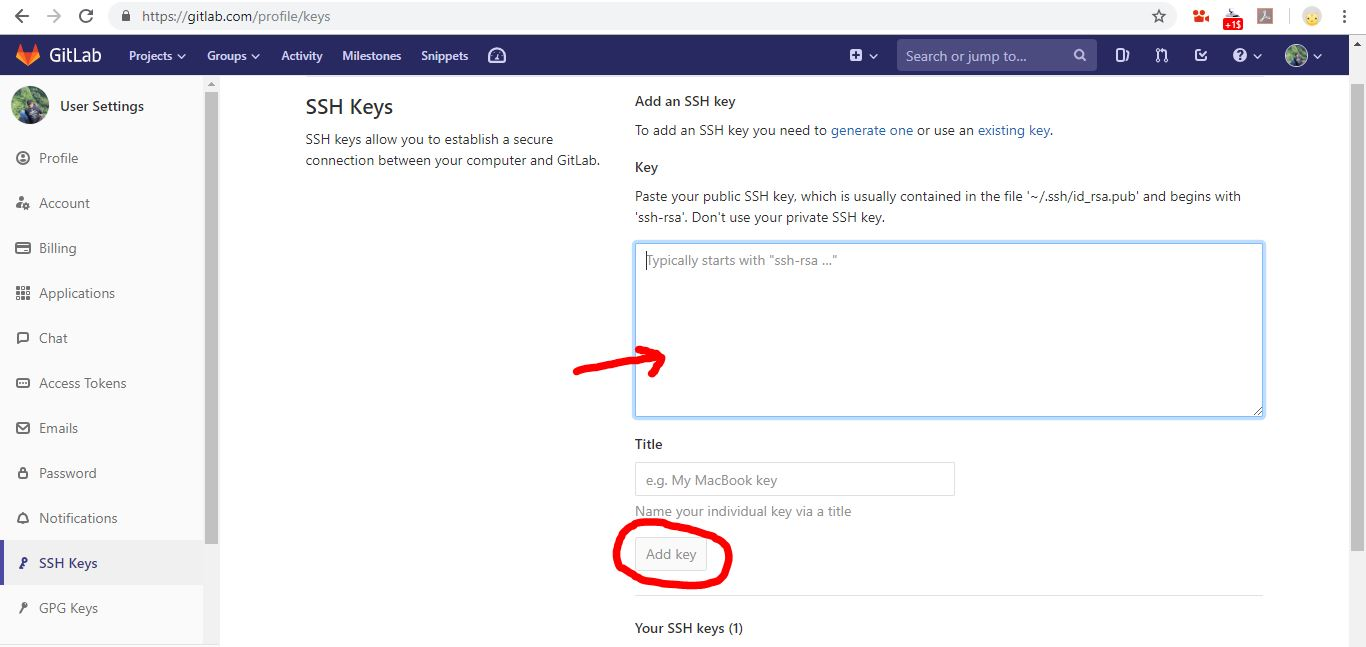
\includegraphics[width=.75\textwidth]{Figures/gitlab/SettingSSH.JPG}}
\caption{Pengisian Form SSH Key Pada Gitlab}
\label{fig:k2}
\end{figure}
\end{enumerate}

\subsection{Membuat Project}
Berikut adalah langkah-langkah yang harus dilakukan dosen untuk membuat suatu project atau repository :
\begin{enumerate}
\item Buka akun gitlab yang sudah kita buat pada \textbf{https://github.com//}
\item Kemudian buka menu projects yang berada di halaman home
\item Setelah itu klik tombol button new project seperti pada gambar berikut \ref{fig:pr1} :
\subitem 
\begin{figure}[!htbp]
\centerline{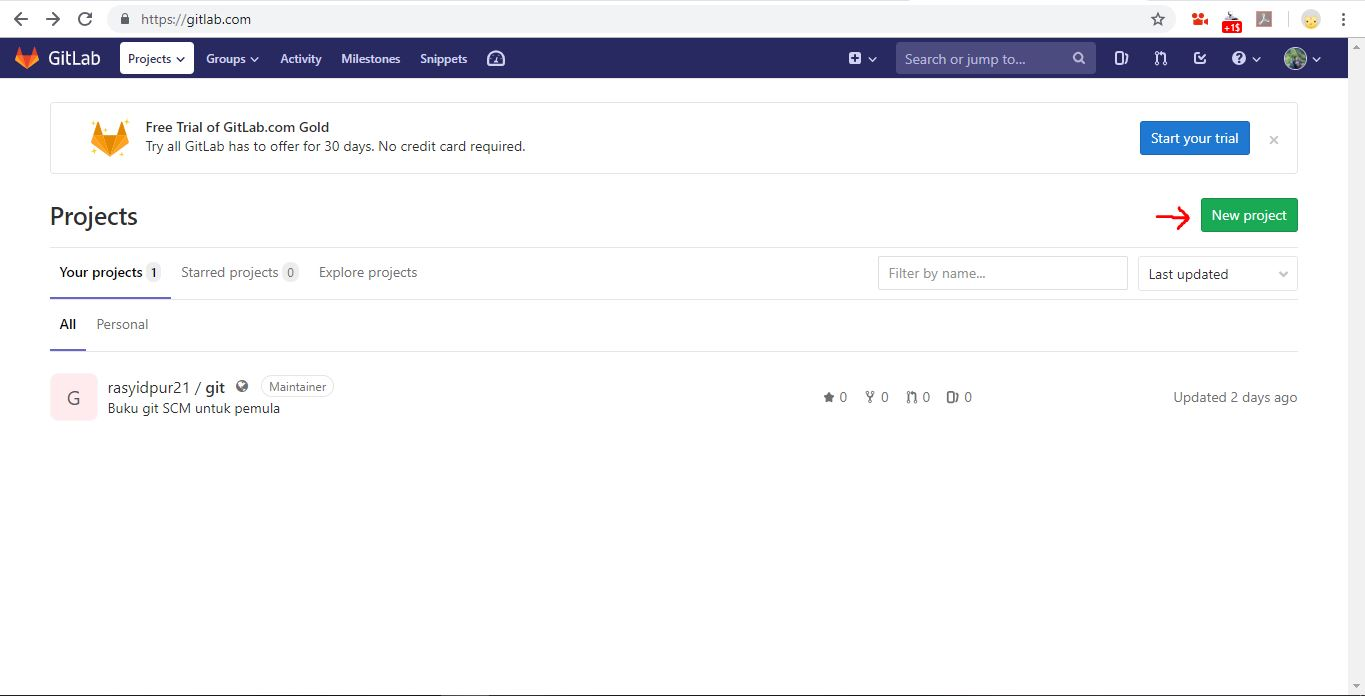
\includegraphics[width=.75\textwidth]{Figures/gitlab/pr1.JPG}}
\caption{Button New Project}
\label{fig:pr1}
\end{figure}
\item Setelah memilih menu new project kita akan diarahkan untuk mengisi data project atau repository apa yang akan kita buat
\item Isi nama project apa yang akan kita buat, disini contoh repository yang kita buat adalah repository \textbf{latihan}
\item Kemudian jangan lupa untuk mengklik radio button \textit{internal} dan radio button \textit{initialize repository with a Readme} seperti pada gambar \ref{fig:pr2} :
\subitem
\begin{figure}[!htbp]
\centerline{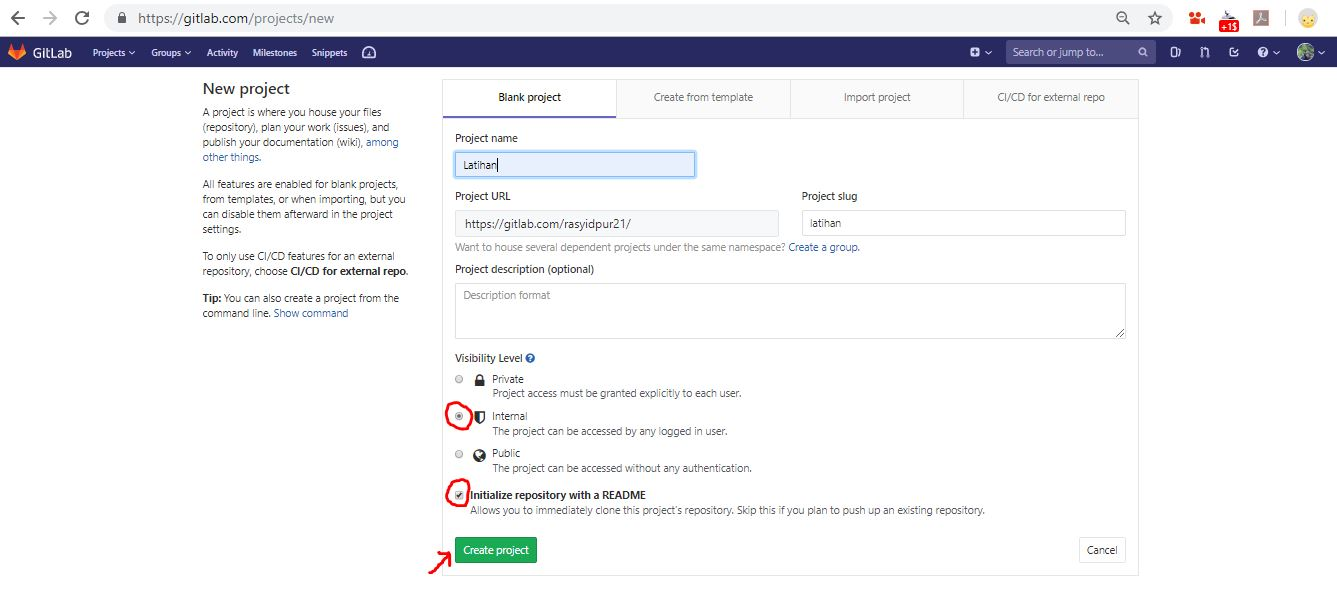
\includegraphics[width=.75\textwidth]{Figures/gitlab/pr2.JPG}}
\caption{Form Create Project}
\label{fig:pr2}
\end{figure}
\item Setelah itu klik tombol button create project seperti gambar \ref{fig:pr2}
\item Setelah kita membuat project, maka repository \textbf{Latihan} telah selesai dibuat
\item Kemudian untuk menyimpan progress project yang akan dibuat didalam repository, kita harus membuat directory 
\item Pada repository latihan klik button seperti yang sudah ditandai pada gambar \ref{fig:pr3}, kemudian klik \textbf{new directory}  
\subitem
\begin{figure}[!htbp]
\centerline{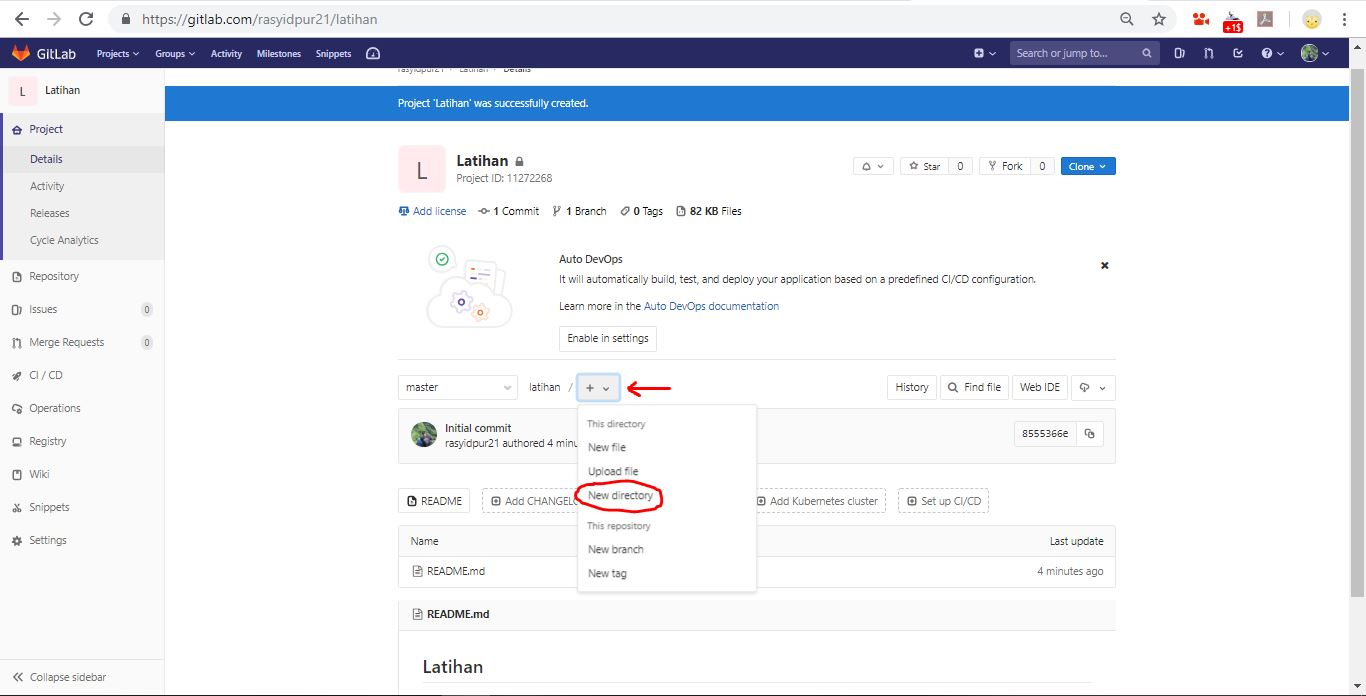
\includegraphics[width=.75\textwidth]{Figures/gitlab/pr3.JPG}}
\caption{Membuat Direktori Baru}
\label{fig:pr3}
\end{figure}
\item Kemudian isi keterangan directory apa yang ingin kita buat, setelah itu klik button \textbf{create button}
\item Pada tutorial ini directory yang akan dibuat adalah directory mahasiswa seperti pada gambar \ref{fig:pr4}
\subitem
\begin{figure}[!htbp]
\centerline{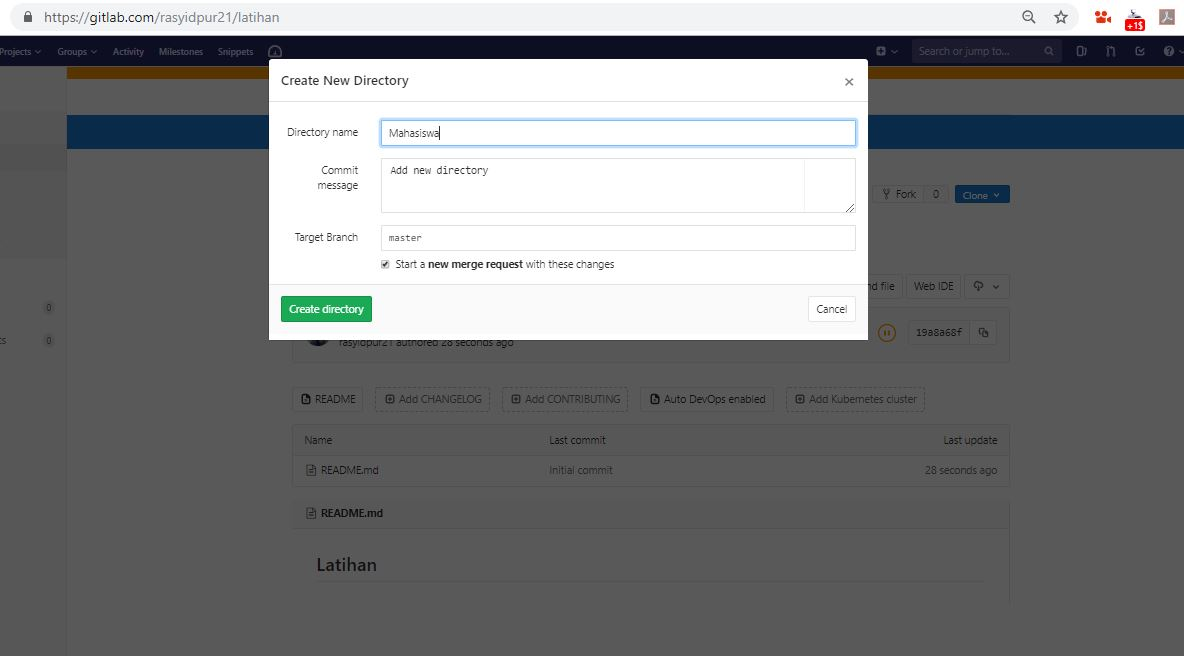
\includegraphics[width=.75\textwidth]{Figures/gitlab/pr4.JPG}}
\caption{Direktori Mahasiswa}
\label{fig:pr4}
\end{figure}
\item Sekarang kita telah berhasil membuat directory \textbf{mahasiswa} pada repository \textbf{Latihan} seperti pada gambar \ref{fig:pr5}
\subitem
\begin{figure}[!htbp]
\centerline{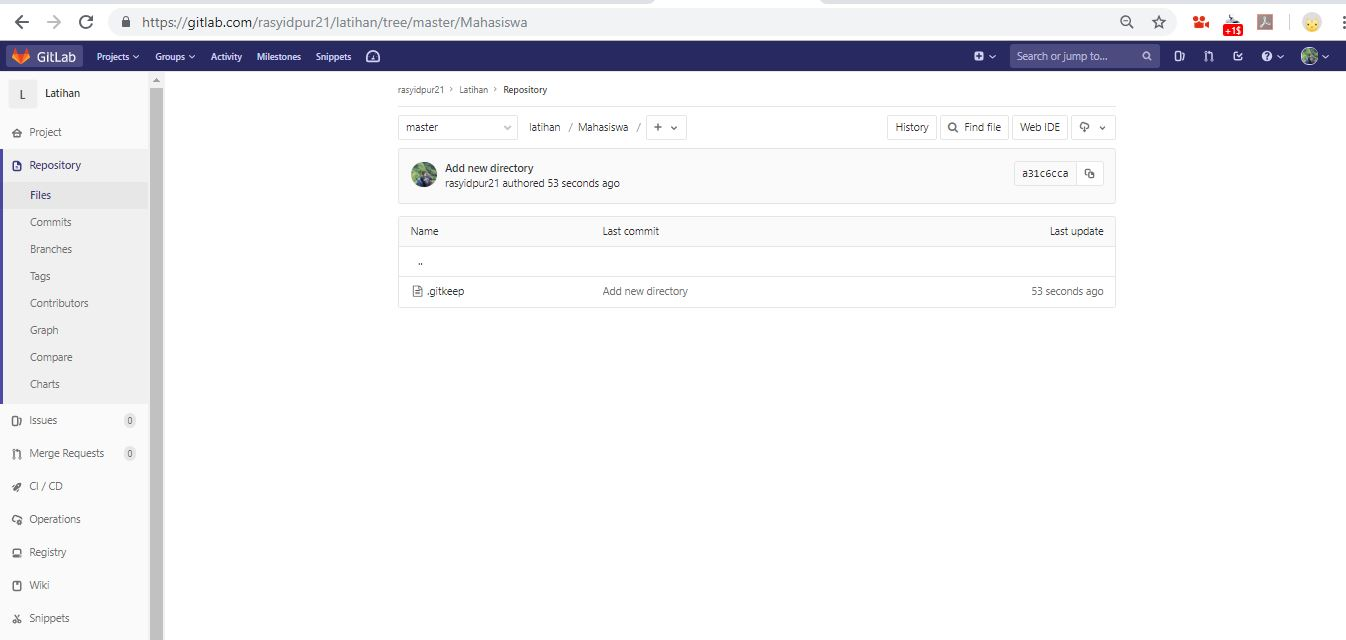
\includegraphics[width=.75\textwidth]{Figures/gitlab/pr5.JPG}}
\caption{Direktori Yang Berhasil Dibuat}
\label{fig:pr5}
\end{figure}
\item Setelah itu kontributor bisa melakukan forking dari repository yang telah kita buat
\item Jika mahasiswa telah melakukan fork pada repository yang sudah dibuat oleh dosen, mahasiswa dapat mengupdate project yang mereka lakukan dengan cara\textbf{pull request} pada directory \textit{Mahasiswa} yang ada didalam repository \textbf{Latihan} 
\item Jika kontributor telah melakukan\textbf{pull request}, pemilik repo dapat melakukan \textbf{merge pull request} dan melihat notifikasi siapa saja yang sudah melakukan pull request dengan mengklik menu \textbf{merge pull request} seperti pada gambar \ref{fig:pr6} :
\subitem
\begin{figure}[!htbp]
\centerline{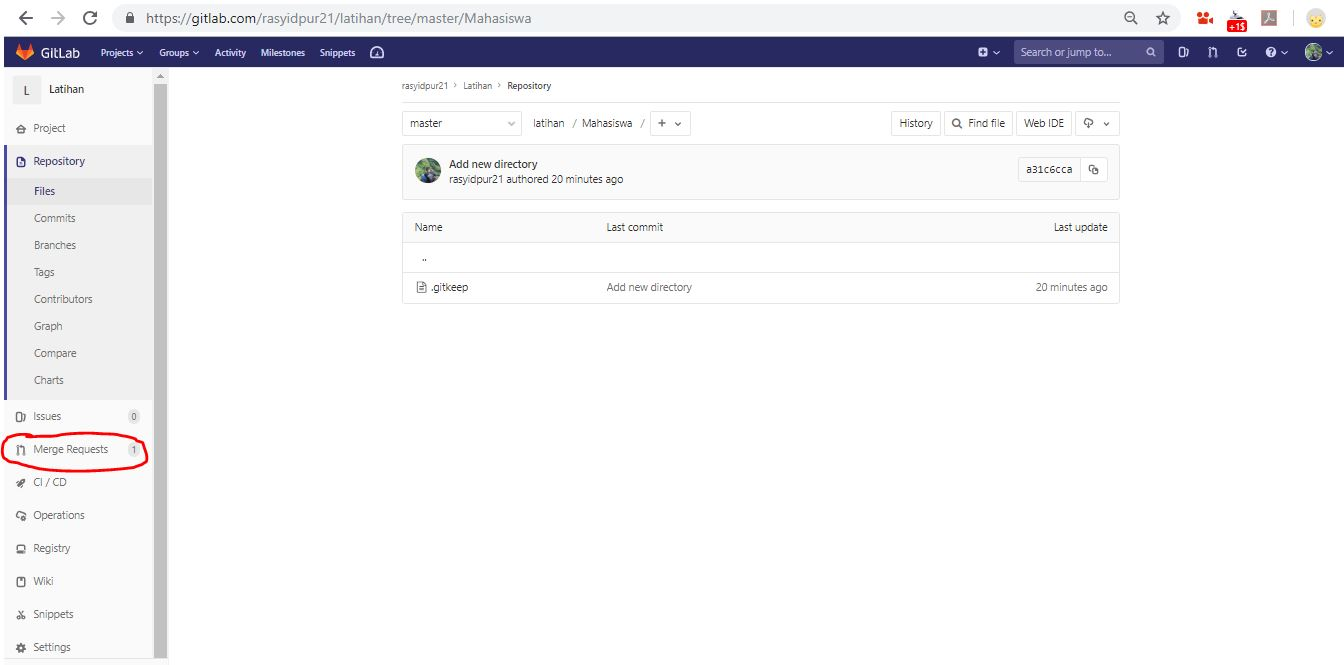
\includegraphics[width=.75\textwidth]{Figures/gitlab/pr6.JPG}}
\caption{Menu Merge Pull Request}
\label{fig:pr6}
\end{figure}
\item Setelah masuk kedalam menu merge pull request, buka file yang berisikan progress yang sudah kontributor lakukan seperti pada gambar \ref{fig:pr7}
\subitem
\begin{figure}[!htbp]
\centerline{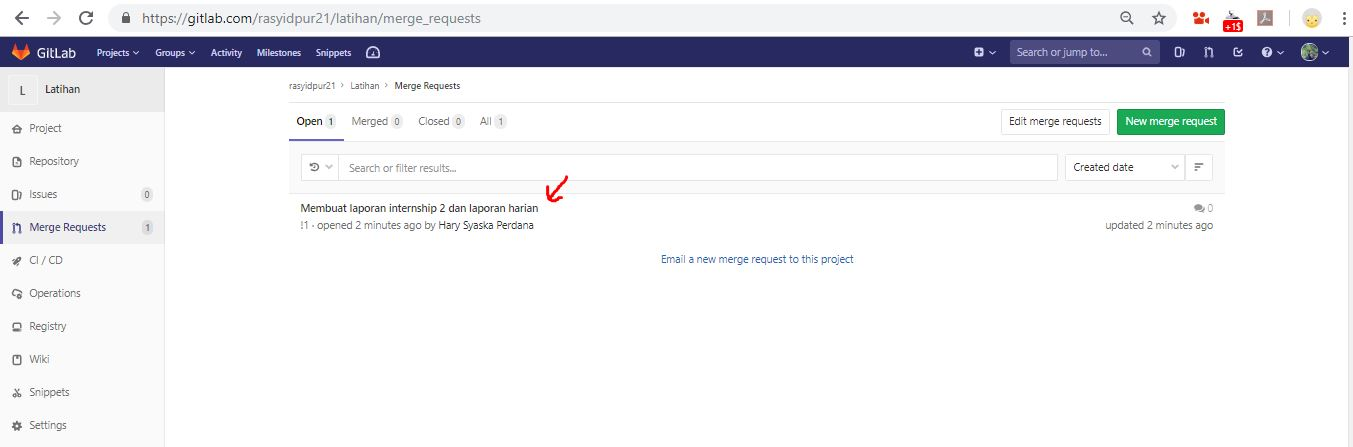
\includegraphics[width=.75\textwidth]{Figures/gitlab/pr7.JPG}}
\caption{Halaman Merge Pull Request}
\label{fig:pr7}
\end{figure}
\item Setelah membuka file maka kita akan diarahkan kepada halaman selanjutnya seperti pada gambar \ref{fig:pr8}
\subitem
\begin{figure}[!htbp]
\centerline{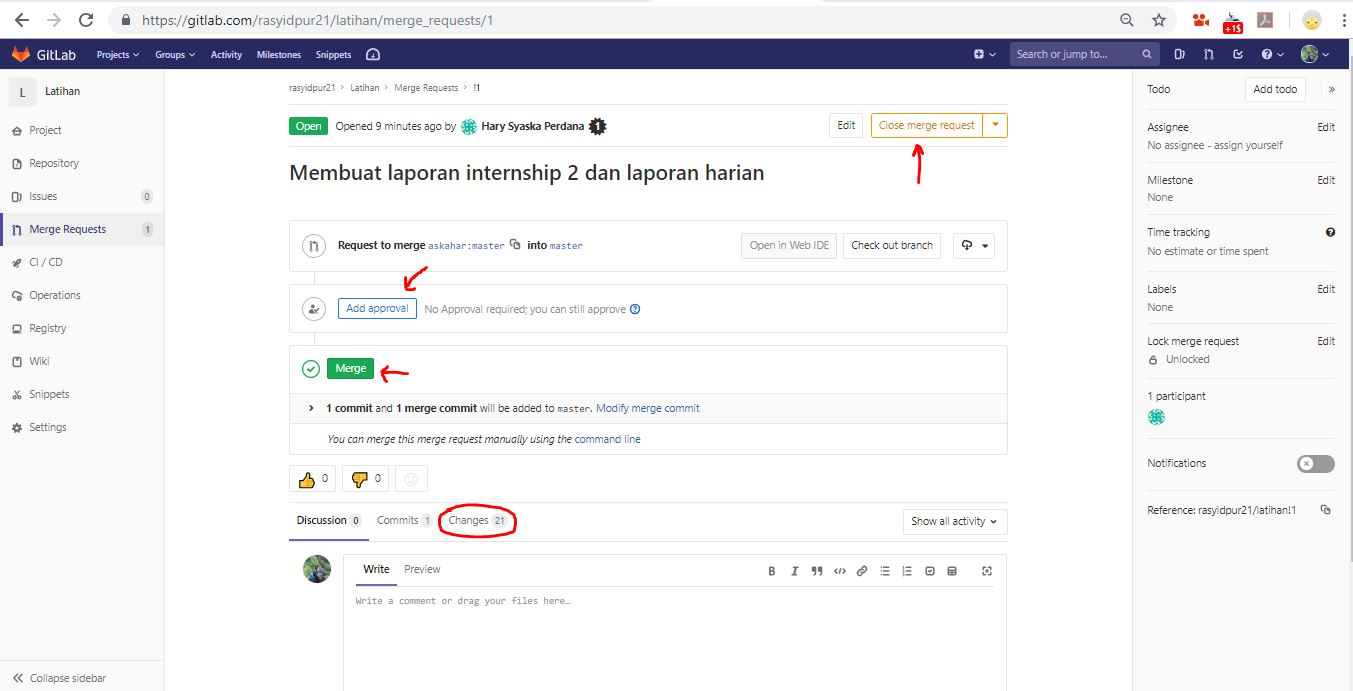
\includegraphics[width=.75\textwidth]{Figures/gitlab/pr8.JPG}}
\caption{Proses Merge Pull Request}
\label{fig:pr8}
\end{figure}
\item Pada gambar \ref{fig:pr8} terdapat beberapa button yang memiliki fungsi yang berbeda-beda
\item Button \textbf{Add Approval} berfungsi agar pemilik repo dapat menambahkan kontributor pada repository latihan untuk melakukan \textit{merge pull request}
\item Button \textbf{Merge} berfungsi untuk meng-approve atau menyetujui perubahan kontribusi yang sudah dilakukan oleh kontributor
\item Button \textbf{Close merge request} berfungsi untuk menutup perubahan kontribusi yang sudah dilakukan oleh mahasiswa atau dengan kata lainnya perubahan yang dilakukan kontributor ditolak
\item Button \textbf{Changes} berfungsi untuk melihat dan menampilkan perubahan apa saja yang sudah kontributor lakukan dari project yang dia kerjakan. Kita dapat mengklik button seperti yang sudah ditandai lingkaran merah pada gambar diatas. Dan perubahan tersebut dapat kita lihat pada gambar \ref{fig:pr9}
\subitem 
\begin{figure}[!htbp]
\centerline{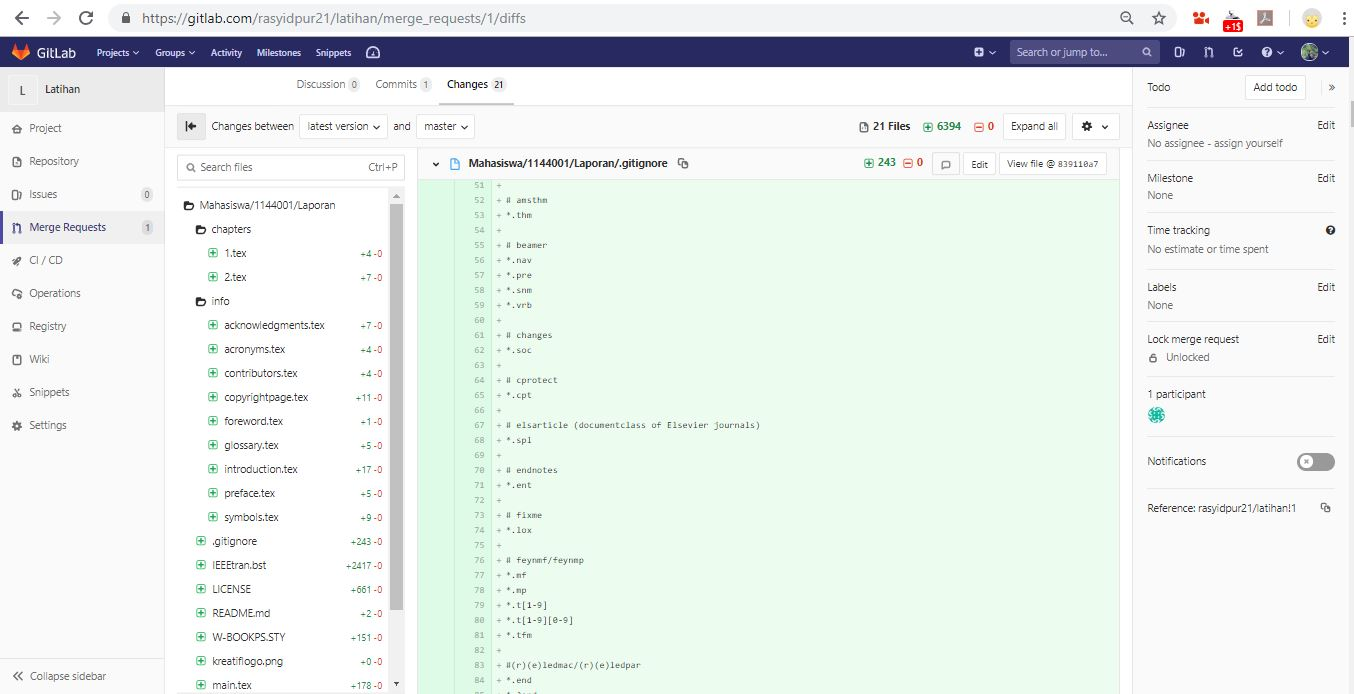
\includegraphics[width=.75\textwidth]{Figures/gitlab/pr9.JPG}}
\caption{Melihat perubahan yang dikaukan kontributor}
\label{fig:pr9}
\end{figure}
\item Jika kita telah melakukan merge pull request maka hasilnya akan seperti pada gambar \ref{fig:pr10}, tepatnya dalam tanda lingkaran merah 
\subitem
\begin{figure}[!htbp]
\centerline{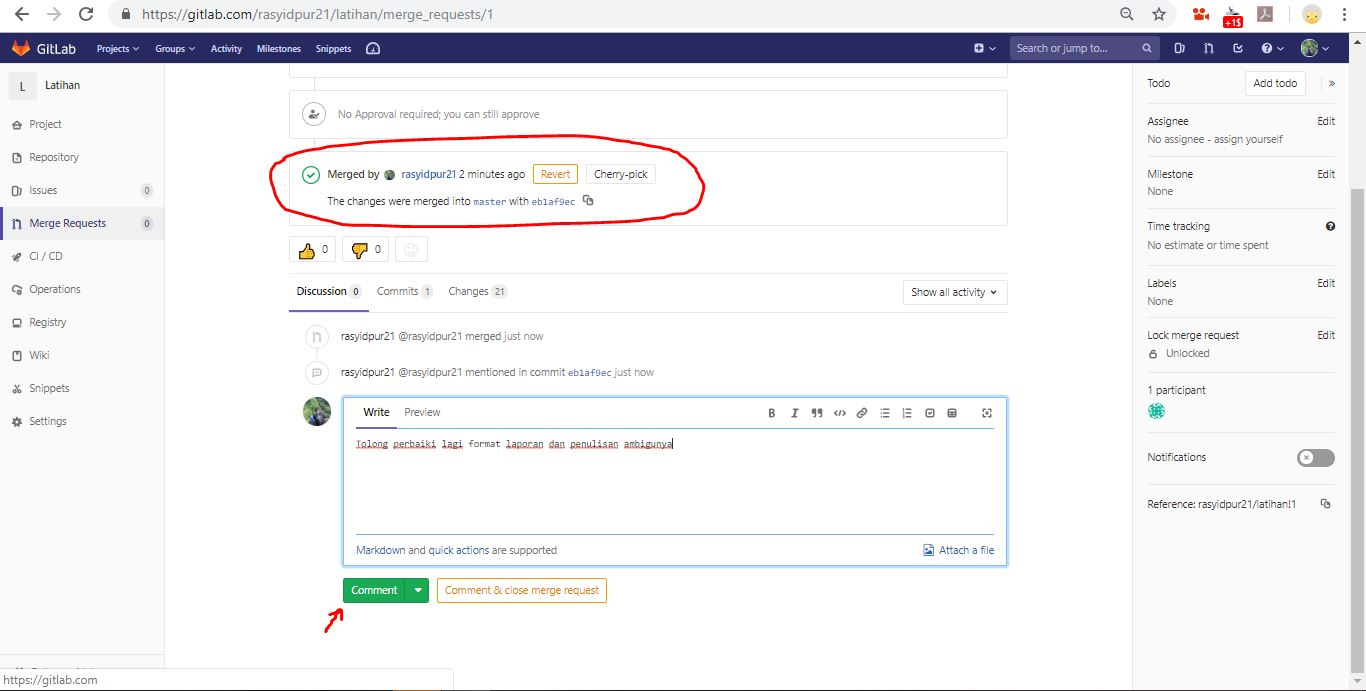
\includegraphics[width=.75\textwidth]{Figures/gitlab/pr10.JPG}}
\caption{Kolom Comment untuk menambahkan komentar}
\label{fig:pr10}
\end{figure}
\item Terakhir pemilik repo juga dapat menambah kan komentar jika ingin merevisi perubahan yang dilakukan kontributor pada kolom komentar seperti pada gambar \ref{fig:pr10}, lalu klik button \textbf{comment} untuk menambahkan komentar
\subitem
\begin{figure}[!htbp]
\centerline{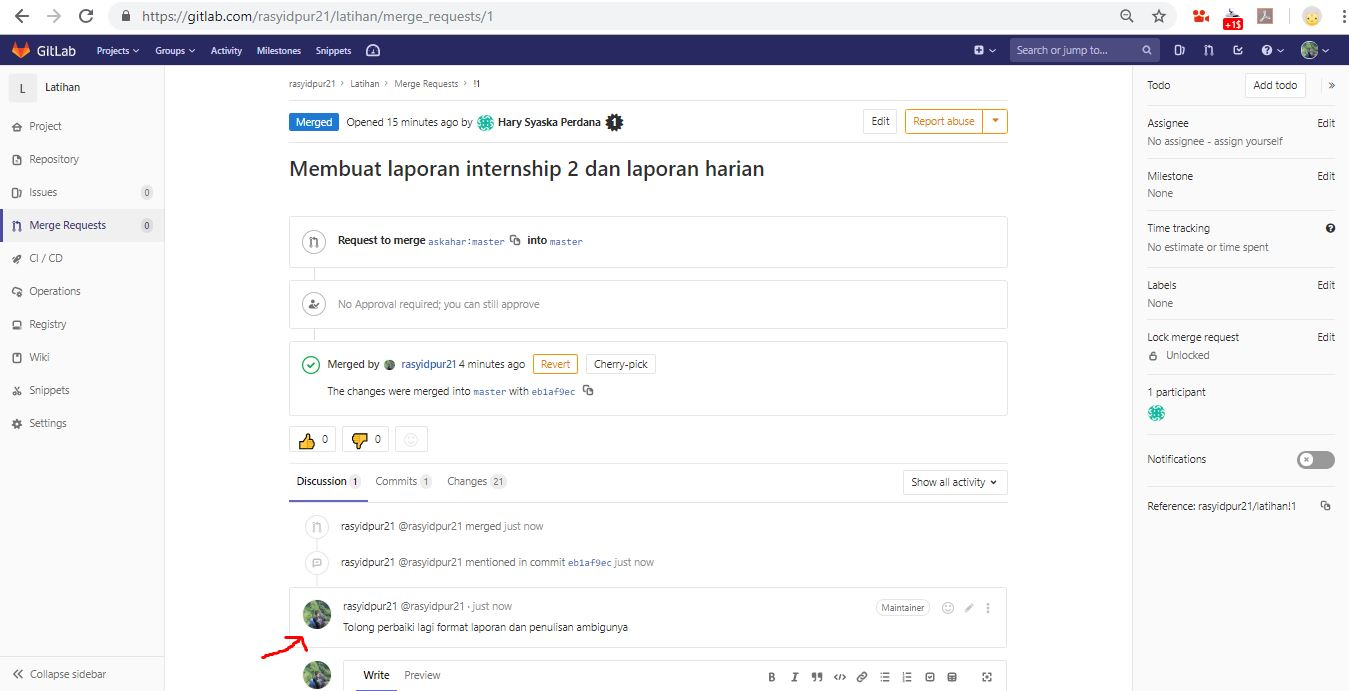
\includegraphics[width=.75\textwidth]{Figures/gitlab/pr11.JPG}}
\caption{Hasil Dari Merge Pull Request}
\label{fig:pr11}
\end{figure}
\end{enumerate}
